\documentclass{article}
\usepackage{amsmath}
\usepackage{graphicx}
\usepackage{listings}
\author{Chang Liu ~\\ chang\_liu@student.uml.edu}
\title{91.673 Advanced Database Systems Homework4}
\begin{document}

\maketitle

\section{Problem 1:Exercise 5.1.2}

\textbf{Exercise 5.1.2}: Compute the PageRank of each page in Fig. 5.7, assuming $\beta$ = 0.8. ~\\
\begin{center}
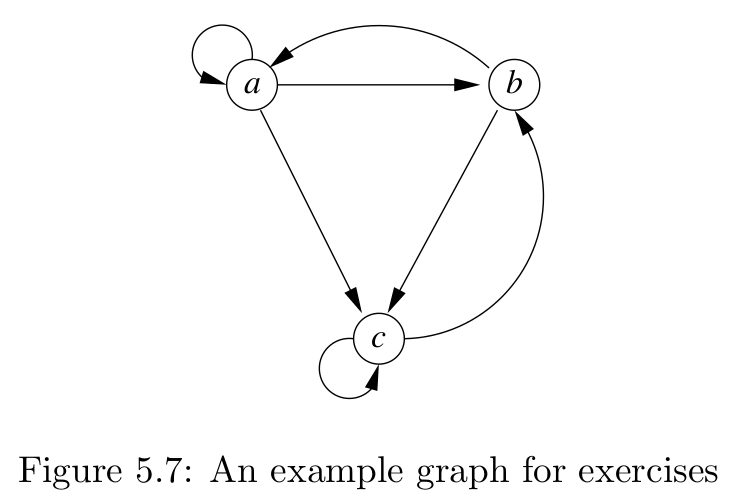
\includegraphics[scale=0.3]{hw3-figure5_7.png}
\end{center}

\textbf{Answer:}

According to the PageRank equation: $$r_j = \sum\limits_{i \rightarrow j}{\beta\frac{r_i}{d_i} + (1-\beta)\frac{1}{N}}$$

First, try to build the stochastic adjacency matrix $M$ using the following relationship about their importance $r_i$
$$r_a = r_b/2 + r_a/3$$
$$r_b = r_a/3 + r_c/2$$
$$r_c = r_a/3 + r_b/2 + r_c/2$$

The we can get:
\begin{equation}
M = \begin{pmatrix} 1/3 & 1/2 & 0 \\ 1/3 & 0 & 1/2 \\ 1/3 & 1/2 & 1/2 \end{pmatrix} 
\end{equation}

Add their result and get the final matrix as follows:

$$r_j = \sum\limits_{i \rightarrow j}{\begin{pmatrix} 1/3 & 7/15 & 1/15 \\ 1/3 & 1/15 & 7/15 \\ 1/3 & 7/15 & 7/15 \end{pmatrix}}$$

Using the equation $r = M * r$, do the iteration multiple times, and then we can get the following result: ~\\
1st iteration: r = (0.33 0.2 0.467) \\
2nd iteration: r = (0.26 0.2 0.52) \\
3rd iteration: r = (0.29 0.18 0.56) \\
... \\
100th iteration: r = (0.2121 0.1515 0.6364) \\

After that it's quite stable, so the PageRank of a is \textbf{0.21}, b is \textbf{0.15}, c is \textbf{0.64} 



\section{Problem 2: Exercise 5.3.1}
\textbf{Exercise 5.3.1}: Compute the topic-sensitive PageRank for the graph of Fig.5.15, assuming the teleport set is:

(a) A only.

(b) A and C.


\begin{center}
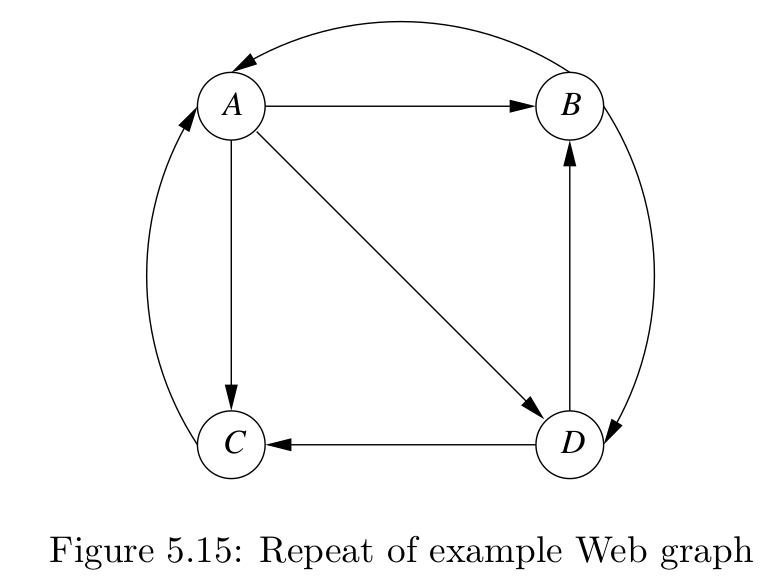
\includegraphics[scale=0.3]{hw4_figure_5_15.png}
\end{center}


\textbf{Answer:}

Here for the topic-sensitive, we should consider the topic when using the random jump, which means that only jumping to the node that related with the topic, the general form is $$v' = \beta{}Mv+(1-\beta)e_s/|S|$$

As the first problem shows, first try to build the matrix M, which is:
$$M = \begin{pmatrix} 0 & 1/2 & 1 & 0 \\ 1/3 & 0 & 0 & 1/2 \\ 1/3 & 0 & 0 & 1/2 \\ 1/3 & 1/2 & 0 & 0\end{pmatrix}$$

(a) For A only, the vector should be (1 0 0 0), as A is the only case, use the equation above with $\beta{}=0.8$, try to start as the vector $v=\begin{matrix} 1 & 0 & 0 & 0\end{matrix}$, since A relates to the topic. NOTE that the initial distribution has no effect on the limit or the final result, doing multiple iterations and the final value reaches:


\begin{center}
v = (0.4286 0.1905 0.1905 0.1905)
\end{center}

so the topic-sensitive PageRank for a, b, c, d is \textbf{0.43}, \textbf{0.19}, \textbf{0.19}, \textbf{0.19} respectively.
~\\

(b) For A and C, the biased vector should be (1/2 0 1/2 0), other functions are the same, using the same method we can get:

\begin{center}
v = (0.3857  0.1714  0.2714 0.1714)
\end{center}

so the topic-sensitive PageRank for a, b, c, d is \textbf{0.39}, \textbf{0.17}, \textbf{0.27}, \textbf{0.17} respectively.

For some details, please refer to my code.


\section{Problem 3: Exercise 6.1.5}

\textbf{Exercise 6.1.5}: For the data of Exercise 6.1.1, what is the confidence of the
following association rules?

(a) $\{5, 7\} \rightarrow  2$.

(b) $\{2, 3, 4\} \rightarrow 5$.

~\\
\textbf{Answer:}

According to the definition of confidence, $$conf(I \rightarrow j) = \frac{support(I \bigcup j)}{support(I)}$$

calculate the probability of the two sets and then we can get the confidence.
~\\

(a) For this case, the probability of showing item 5 and 7 in the same basket is that the basket number can be divided by 5 AND 7, so it can only be 35 and 70 in these two cases. $p(support(I)) = 2/100$.

And the probability of showing item 2, 5, 7 in the same time can only be the case that basket number is 70, the so probability is $p(support(I \bigcup j)) = 1/100$.

According to the above equation, the confidence should be 0.5 after their division.

~\\
(b) Using the same method, in the set I, the basket can be $\{$12, 24, 36, 48, 60, 72, 84, 96$\}$, so probability is $p(support(I)) = 8/100$. And the probability of I with j is $p(support(I \bigcup j)) =  1/100$, as the basket can only be 60, so the confidence in this case should be 1/8 = 0.125.



\section{Problem 4: Exercise 6.2.6 (a)}

\textbf{Exercise 6.2.6}: Apply the A-Priori Algorithm with support threshold 5 to the data of:

(a) Exercise 6.1.1.

~\\
\textbf{Answer:}

We can use the following graphs to help us describe how to use the A-Priori Algorithm:

\begin{center}
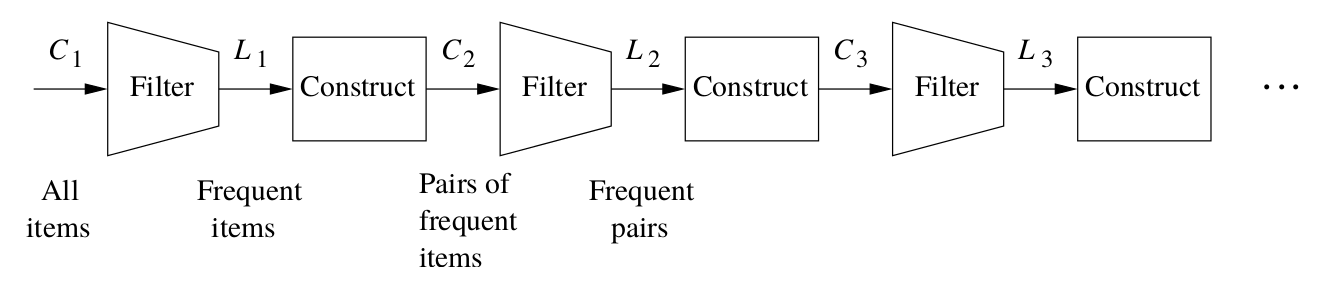
\includegraphics[scale=0.3]{hw4_p5.png}
\end{center}

Here the threshold is 5, so we just need to go through the structure and the item will occur more than 5 times. First define some terminology:

1. $C_k$ is the set of candidate itemsets of size k – the itemsets that we must count in order to determine whether they are in fact frequent.

2. $L_k$ is the set of truly frequent itemsets of size k.

~\\
The methods are as follows:

For the data in the Exercise 6.1.1, first for all items, go through the first Filter, this will find the truly frequent itemsets $L_1$ from $C_1$, which means that there is only 1 item in each set. That will generate some baskets that only contain 1 item but this one item is frequent in all the candidates. For all the items, due to the threshold, it will contain items that no larger than 20, otherwise it will occur less than 5 times, because 20 * 5 = 100. For example, item 21 can only be occurred in basket $\{$21, 42, 63, 84$\}$, that's less than 5, so for any number larger than 20, it will always be less than 5, in this way, we know $L_1$ only contains item $\{$1, 2, 3, 4, ... 20$\}$.

Then using this frequent item in $L_1$, we construct the two-item sets, forming the candidate of $C_2$, and going through the Filter to find the frequent itemset $L_2$, this will generate the itemsets that are frequent in 2-elements.

In the same way, for 3-elements, just combin the $L_2$ and $L_1$, that will construct all the candidates for $C_3$, then using the Filter to find the frequent one, will will yield the $L_3$...

Until we find the frequent itemsets $L_5$, repeat the above process using same method.

for size k = 1, since $\{$1$\}$ to $\{$20$\}$ all contains in the frequent.

for size k = 2, it should contain $\{$1,2$\}$, $\{$1,3$\}$, ... $\{$1,20$\}$, $\{$2,3$\}$, ... $\{$2,10$\}$, $\{$2,12$\}$, $\{$2,14$\}$... $\{$2,20$\}$ ... $\{$10,20$\}$.

for size k = 3, it adds 1-element to the k = 2 set, so it should contain $\{$2,3,4$\}$, $\{$2,3,6$\}$, ... $\{$6,9,18$\}$

for size k = 4, the set should be $\{$2,3,4,6$\}$, $\{$2,3,4,12$\}$ ... $\{$4,5,10,20$\}$

for size k = 5, the set should be $\{$2,3,4,6,12$\}$, $\{$2,3,6,9,18$\}$, $\{$2,4,5,10,20$\}$

for size k = 6, add 1 to all except 1 is already, $\{$1,2,3,4,6,12$\}$, $\{$1,2,3,6,9,18$\}$, $\{$1,2,4,5,10,20$\}$.

So these three sets are the max size frequent itemsets.


\section{Problem 5: Exercise 7.3.1}


\textbf{Exercise 7.3.1}: For the points of Fig. 7.8, if we select three starting points using the method
of Section 7.3.2, and the first point we choose is (3,4), which other points are selected.

\begin{center}
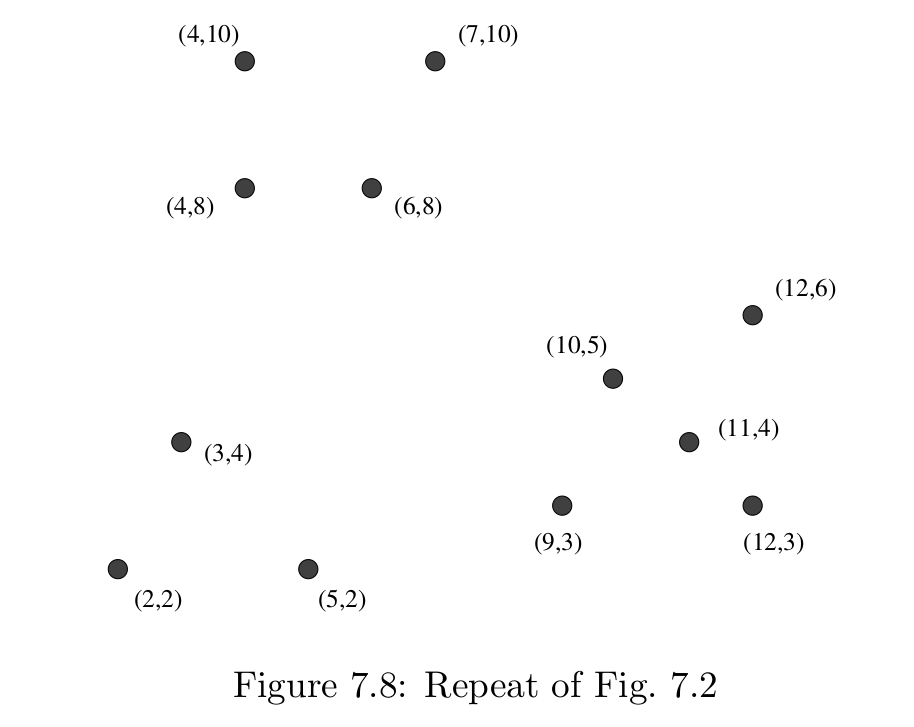
\includegraphics[scale=0.3]{hw4_Figure_7_8.png}
\end{center}

~\\
\textbf{Answer:}

According to the method in Section 7.3.2, we need to pick the points that are as far way for other points as possible. So the other points should be chosen following this rule.

First, we pick a point that is furthest from point (3,4), which is the point \textbf{(12, 6)}. Then among all the other points in the remaining, we will find the point that are most far from these two points.

Using the attached code, we will find that the last point should be \textbf{((7, 10)}, the work should just calculate the distance, get the minimal from the two distance that the point is from point A and point B, do that process for all the points, and then find the biggest one, the corresponding point is just what we need.

So the remaining points are \textbf{(12,6)}, \textbf{(7, 10)}.

\section{Appendix: Code}

\textbf{ex2.m}

\begin{lstlisting}[frame=single]
M = [0 1/2 1 0; 1/3 0 0 1/2; 1/3 0 0 1/2; 1/3 1/2 0 0]; 
v = [1 0 0 0]'; % initial value no effects for final result
%cons = [1 0 0 0]'; % for case a), has different bias
cons = [0.5 0 0.5 0]'; % for case b), 

for i = 1:100
    v = 0.8 * M * v + 0.2 * cons;
end
% ends, v is the final vector for (a,b,c,d)
\end{lstlisting}



\textbf{ex5.py}

\begin{lstlisting}[frame=single]
#!/usr/bin/env python
"""
function: pick_kmean_point()
descripition: find the most and second furthest point
"""
import math

# given first point, find the other one furthest from it
point1 = (3, 4)
points = [(2,2), (5,2), (9,3), (12,3), (11,4),\
        (12,6), (10,5), (4,8), (6,8), (4,10), (7, 10)]

# given two points, find the remaining one furthest
point_set = [(3,4), (12,6)]
other_points = [(2,2), (5,2), (9,3), (12,3),\
        (11,4), (7,10), (10,5), (4,8), (6,8), (4,10)]

def find_most_distant(point, points):
    max_distance = 0
    marker = ()
    for p in points:
        # here we just use dst's square to represent
        distance = math.sqrt(math.pow(p[0]-point[0], 2) \
                + math.pow(p[1]-point[1], 2))
        if distance > max_distance:
            max_distance = distance
            marker = p
    print marker

def find_last_point(points, other_points):
    max_distance = 0
    marker = ()
    # for limited time, I don't use loop for points
    for p in other_points:
        dst1 = math.sqrt(math.pow(p[0]-points[0][0], 2) \
                + math.pow(p[1]-points[0][1], 2))
        dst2 = math.sqrt(math.pow(p[0]-points[1][0], 2) \
                + math.pow(p[1]-points[1][1], 2))
        distance = min(dst1, dst2)
        if distance > max_distance:
            max_distance = distance
            marker = p
    print marker

find_most_distant(point1, points)
find_last_point(point_set, other_points)
\end{lstlisting}


\end{document}

